\section{Zusatzfunktionen}
Dieses Kapitel widmet sich den Eastereggs des Moduls \avl.\\
Sollten Sie sich lieber selber gerne auf die Suche nach diesen Zusatzfunktionen machen wollen, so �berspringen Sie besser dieses Kapitel.\\
F�r alle Anderen folgt nun eine �bersicht zum Baumnavigator und dem Beamermodus.

\subsection{Navigator}
Der Navigator ist eine kleine, versteckte Zusatzfunktion, die die Arbeit mit gro�en B�umen erheblich vereinfachen kann. Er stellt eine willkommene Hilfe f�r das Scrollen der Zeichenfl�che dar, ist aber nicht so einfach zu finden.
\begin{itemize}
	\item Wenn der Baum, der auf der Zeichenfl�che angezeigt wird, zu gro� f�r diese wird, so erscheinen Schiebebalken, mit denen Sie den Bildausschnitt verschieben k�nnen.
	\item Klicken Sie nun auf das kleine Quadrat in der rechten unteren Ecke der Zeichenfl�che, genau zwischen den beiden Schiebebalken. Halten Sie dabei die linke Maustaste gedr�ckt.
	\item Eine kleine �bersichtskarte des Baumes mit einem Ausschnittfenster erscheint. Bewegen Sie die Maus (mit gedr�ckter Taste) und das Ausschnittfenster, das den Bildschirminhalt der Zeichenfl�che repr�sentiert, folgt Ihren Bewegungen.
\end{itemize}
\bigskip
\begin{center}
	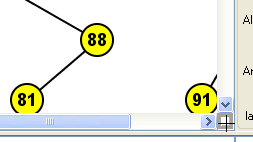
\includegraphics[scale=0.7]{\pfad avl/navigator1} \hfill
	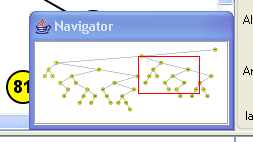
\includegraphics[scale=0.7]{\pfad avl/navigator2} \\
	Ein Klick auf das kleine K�stchen... \hfill ...�ffnet den Navigator!
\end{center}

\subsectionicon{Beamermodus}{avl/icon_beamer}
Der Beamermodus ist in erster Linie f�r die Pr�sentation in Vorlesungen oder �hnlichen Veranstaltungen gedacht. Ist dieser Modus aktiv, so werden die Knoten des Baumes und die Eintr�ge des Logbuches vergr��ert dargestellt. Der Algorithmustext aus dem Skript von Prof. Vogler bleibt dabei unver�ndert, weil davon ausgegangen wird, dass die interessierten Studenten der Vorlesung �ber ein (eventuell aktuelleres) Skript verf�gen.\\
Sie erreichen den Beamermodus �ber den Men�punkt \textsc{<\avl>} $\rightarrow$ \textsc{<Beamermodus>}. Ist der Modus aktiv, so erscheint neben diesem Men�eintrag ein H�kchen. Um den Modus wieder auszuschalten, entfernen Sie einfach den Haken per Klick.
\bigskip
\centerpic{avl/beamermenu}{0.5}{Das Men� \textsc{<\avl>} mit dem Eintrag \textsc{<Beamermodus>}}

\newpage